\chapter{Hawkes Process Modeling and Inference Details}
\label{AppendixB}

\section{Inference details}
\subsection{Derivation of conjugate prior updates}
By combining
Equations~\ref{eq:poisson_lkhd}~and~\ref{eq:hawkes_likelihood} of the
main text, we can write the joint likelihood, with the auxiliary
parent variables, as,
\begin{multline}
  \label{eq:complete_likelihood}
  \Pr(\{s_n,c_n,z_n\}^N_{n=1},\given \{\lambda_{0,k}(t)\}^K_{k=1}, \{h_{k,k'}(\Delta t)\}_{k,k'}) = \\
  \prod^K_{k=1} \bigg[
  \exp\left\{ -\int_0^T \lambda_{0,k}(\tau)\mathrm{d}\tau \right\} \,
  \prod^N_{n=1}
   \lambda_{0,k}(s_n)^{\delta_{c_n,k}\delta_{z_n,0}} \bigg]\\
  \quad\times \prod_{n=1}^N\prod_{k'=1}^K \bigg[
  \exp\left\{-\int^T_{s_n} h_{c_n,k'}(\tau - s_n)\mathrm{d}\tau \right\}\\
  \prod^N_{n'=1} h_{c_n,c_{n'}}(s_{n'}-s_n)^{\delta_{c_{n'},k'}\delta_{z_{n'},n}}\bigg].
\end{multline}
The first line corresponds to the likelihood of the background
processes; the second and third correspond to the likelihood of the
induced processes triggered by each spike.

To derive the updates for weights, recall from
Equation~\ref{eq:ir_decomp} of the main text that~${W_{k,k'}}$ only
appears in the impulse responses for which~${c_n=k}$
and~${c_{n'}=k'}$. so we have,
\begin{align*}
&p(W_{k,k'}\given \{s_n,c_n,z_n\}^N_{n=1},\ldots) \\
&\propto\prod_{n=1}^N\left[ \exp\left\{-\int^T_{s_n} h_{k,k'}(\tau - s_n)\mathrm{d}\tau \right\}\right.\\
&\quad\quad\left.\prod_{n'=1}^N h_{k,k'}(s_{n'}-s_n)^{\delta_{c_{n'},k'}\delta_{z_{n'},n}}\right]^{\delta_{c_n,k}} \times p(W_{k,k'})\\
&=\prod_{n=1}^N\left[ \exp\left\{-\int^T_{s_n} A_{k,k'}W_{k,k'}g_{k,k'}(\tau - s_n)\mathrm{d}\tau \right\}\right.\\
&\quad\quad\left.\prod_{n'=1}^N \left(A_{k,k'}W_{k,k'}g_{k,k'}(s_{n'}-s_n)\right)^{\delta_{c_{n'},k'}\delta_{z_{n'},n}}\right]^{\delta_{c_n,k}}\\
&\quad\quad\quad\times p(W_{k,k'}).
\end{align*}
If~${A_{k,k'}=1}$ and we ignore spikes after~${T-\Delta
  t_{\mathsf{max}}}$, this is approximately proportional to
\begin{align*}
&\exp\left\{-W_{k,k'}N_k\right\} W_{k,k'}^{N_{k,k'}} p(W_{k,k'}),
\end{align*}
where
\begin{align*}
N_{k}=\sum_{n=1}^N \delta_{c_n,k},\;\text{and}\;
N_{k,k'}=\sum_{n=1}^N\sum_{n'=1}^N \delta_{c_n,k}\delta_{c_{n'},k'}\delta_{z_{n'},n}.
\end{align*}
When~${p(W_{k,k'})}$ is a gamma distribution, the conditional
distribution is also gamma. If~${A_{k,k'}=0}$, the conditional
distribution reduces to the prior, as expected.

Similar conjugate updates can be derived for constant background rates
and the impulse response parameters, as stated in the main text.

\subsection{Log Gaussian Cox Process background rates}
In the Trades on the S\&P100 and the Gangs of Chicago datasets, it was
crucial to model the background fluctuations that were shared among
all processes. However, if the background rate is allowed to vary at
time scales shorter than~${\Delta t_{\textsf{max}}}$ then it may
obscure interactions between processes. To prevent this, we sample the
Log Gaussian Cox Process (LGCP) at a sparse grid of~$M+1$ equally
spaced points and linearly interpolate to evaluate the background rate
at the exact time of each event. We have,
\begin{align*}
\by=\left\{\hat{y}\left(\frac{mT}{M}\right)\right\}_{m=0}^M \sim \mathcal{GP}(\boldsymbol{0},K(t,t')).
\end{align*}
Then,

\begin{align*}
\left\{\hat{\lambda}_{0,k}\left(\frac{mT}{M}\right)\right\}_{m=0}^M &= \mu_k + \alpha_k\exp\left\{\hat{y}\left(\frac{mT}{M}\right)\right\},
\end{align*}
and~${\lambda_{0,k}(s_n)}$ is linearly interpolated between the rate
at surrounding grid points.

\begin{comment}
\begin{align*}
\lambda_{0,k}(s_n) &= (1-f_n)\hat{\lambda}_{0,k}\left(\frac{\ell_nT}{M}\right) + f_n\hat{\lambda}_{0,k}\left(\frac{u_nT}{M}\right),
\end{align*}
where
\begin{align*}
\ell_n = \left\lfloor\frac{s_nM}{T}\right\rfloor,\;
u_n = \left\lceil\frac{s_nM}{T}\right\rceil,\;\text{and}\;
f_n = \frac{\frac{s_nM}{T}-\ell_n}{u_n-\ell_n}.
\end{align*}
\end{comment}
The equally spaced grid allows us to calculate the integral using the
trapezoid quadrature rule. We use elliptical slice sampling
\cite{Murray-2010} to sample the conditional distribution of the
vector ~$\by$.

Kernel parameters are set empirically or with prior knowledge. For
example, the period of the kernel is set to one day for the S\&P100
dataset and one year for the Gangs of Chicago dataset since these are
well-known trends. The scale and offset parameters have log Normal
priors set such that the maximum and minimum homogeneous event counts
in the training data are within two standard deviations of the
expected value under the LGCP background rate. That is, the background
rate should be able to explain all of the data without any
observations if there is no evidence for interactions.

\subsection{Priors on hyperparameters}
When possible, we sample the parameters of the prior
distributions. For example, in the Erd\H{o}s-Renyi graph model we
place a~${\mathrm{Beta}(1,1)}$ prior on the sparsity~$\rho$. For the
latent distance model, we place a log normal prior on the
characteristic length scale~${\tau}$ and sample it using Hamiltonian
Monte Carlo.

For all of the results in this paper, we fixed the prior on the
interaction kernel,${~g(\Delta t)}$ to a weak Normal-Gamma
distribution with parameters ${\mu_\mu^0=-1.0}$, ${\kappa_\mu^0=10}$,
${\alpha_\tau^0=10}$, and ${\beta_\tau^0=1}$.

\paragraph{Scale of gamma prior on weights.}
For real data, we place an uninformative prior on the weight
distribution. The gamma distribution is parameterized by a shape
$\alpha_W^0$ and an inverse scale or rate $\beta_W^{0}$. The shape
parameter~${\alpha_W^0}$ is chosen by hand (typically we
use~${\alpha_W^0=2}$), but the inverse scale parameter~${\beta_W^0}$
is sampled. We may not know a proper scale a priori, however we can
use a scale-invariant Jeffrey's prior to infer this parameter as
well. Jeffrey's prior is proportional to the square root of the Fisher
information, which for the gamma distribution is
\begin{align*}
  \Pr(\beta_W^0) \propto \sqrt{I(\beta_W^0)} = \frac{\sqrt{\alpha_W^0}}{\beta_W^0}.
\end{align*}
Hence the posterior is 
\begin{align*}
&\Pr(\beta_W^0 \given \{\{W_{k,k'}\}\} ) \propto \\
&\frac{\sqrt{\alpha_W^0}}{\beta_W^0}\prod_{k=1}^K\prod_{k'=1}^K \frac{(\beta_W^0)^{\alpha_W^0}}{\Gamma(\alpha_W^0)} W_{k,k'}^{\alpha_W^0-1}e^{-\beta_W^0 W_{k,k'}} \\
%&=\frac{\sqrt{\alpha_W^0}}{\Gamma^{K^2}(\alpha_W^0)} (\beta_W^0)^{K^2\alpha_W^0-1} e^{-\beta_W^0\sum_{k=1}^{K}\sum_{k'=1}^K W_{k,k'}}\\
%&\quad\quad\times\prod_{k=1}^K\prod_{k'=1}^K W_{k,k'}^{\alpha_W^0-1} \\
&\propto (\beta_W^0)^{K^2\alpha_W^0-1} \exp\left\{-\beta_W^0 \sum_{k=1}^{K}\sum_{k'=1}^K W_{k,k'}\right\}.
\end{align*}
This is a gamma distribution with parameters,
\begin{align*}
\beta_W^0\sim\distGamma(K^2\alpha_W^0,\sum_{k=1}^K\sum_{k'=1}^K W_{k,k'}).
\end{align*}


\section{Synthetic test details}
We generated~${T=1000}$s of events for each synthetic network. The
average number of spikes was 25,732~$\pm$~9,425. Network 6, the only
network for which the GLM outperformed the network Hawkes model in the
event-prediction test, was an outlier with 44,973 events. For event
prediction, we trained on the first 900 seconds and tested on the last
100 seconds of the data. We ran our Markov chain for 2500 iterations
and computed the posterior probabilities of~$\bA$ and~$\bW$ using the
last 500 samples.

A simple alternative to the Hawkes model is to look at
cross-correlation between the event times. First, the event times are
binned into an array~$\hat{\bs}_k$ of length~$M$. Let~${(\hat{\bs}_k
  \star \hat{\bs}_{k'})[m]}$ be the cross-correlation
between~$\hat{\bs}_k$ and~$\hat{\bs}_{k'}$ at discrete time
lag~$m$. Then,~${W_{k,k'}=\sum_{m=0}^{\Delta
    t_{\mathsf{max}}M/T}(\hat{\bs}_k \star \hat{\bs}_{k'})[m]}$
provides a simple measure of directed, excitatory interaction that can
be thresholded to perform link prediction.

Additionally, we compare the network Hawkes process to the generalized
linear model for point processes, a popular model in computational
neuroscience \cite{Paninski-2004}. Here, the event counts are modeled
as ${\hat{s}_{k,m}\sim\text{Poisson}(\lambda_{k,m})}$. The mean
depends on external covariates and other events according to
\begin{align*}
  \lambda_{k,m} &= \exp\left\{ \balpha_k^T\by_m + \sum_{k'=1}^K\sum_{b=1}^B \beta_{k,k',b} (g_{b}\ast \hat{s}_{k'})[m ]\right\},
\end{align*}
where $\by_m$ is an external covariate at time~$m$, $\{g_b(\Delta
m)\}_{b=1}^B$ are a set of basis functions that model impulse
responses, and $\balpha$ and $\bbeta$ are parameters to be
inferred. Under this formulation the log-likelihood of the events is
concave function of the parameters and is easily maximized. Unlike the
Hawkes process, however, this model allows for inhibitory
interactions.

For link prediction,~${\sum_b \beta_{k,k',b}}$ provides a measure of
directed excitatory interaction that can be used to compute an ROC
curve. In our comparisons, we used~${\by_m\equiv 1}$ to allow for
time-homogeneous background activity and set~${\{g_b(\Delta m)\}}$ to
the top~${B=6}$ principal components of a set of logistic normal
impulse responses randomly sampled from the Hawkes prior.

We used an L1 penalty to promote sparsity in the parameters of the
GLM, and chosen the penalty using cross validation on the last 100
seconds of the training data.

\begin{table}[h!]
  \begin{center}
    \begin{tabular}{|l|c|}
      \hline
      \textbf{Model} & \textbf{Relative prediction improvement} \\
      \hline
      Network Hawkes & 100\% \\
      Standard Hawkes & 59.2$\pm$14.2\% \\
      GLM & 71.6$\pm$9.2\%\\
      \hline
    \end{tabular}
  \end{center}
  \caption[Predictive log likelihood for synthetic data]{Relative
    improvement in predictive log likelihood over a homogeneous
    Poisson process baseline. Relative to the network Hawkes, the
    standard Hawkes and the GLM yield significantly less predictive
    power.}
  \label{tab:rel_pred_ll}
\end{table}

Figure~\ref{fig:synth_pred_ll} of the main text shows the predictive
log likelihoods for the Hawkes model with the correct Erd\"os-Renyi
prior, the standard Hawkes model with a complete graph of
interactions, and a GLM. On all but network 6, the network Hawkes
model outperforms the competing models in terms of predictive log
likelihood. Table~\ref{tab:rel_pred_ll} shows the average predictive
performance across sample nextworks. The standard Hawkes and the GLM
provide only 59.2\% and 71.6\%, respectively, of this predictive
power.

\section{Trades on the S\&P100 model details}
We study the trades on the S\&P~100 index collected at 1s intervals
during the week of Sep.~28 through Oct.~2,~2009. We group both
positive and negative changes in price into the same process in order
to measure overall activity. Another alternative would be to generate
an ``uptick'' and a ``downtick'' process for each stock.  We ignored
trades outside regular trading hours because they tend to be outliers
with widely varying prices. Since we are interested in short term
interactions, we chose~${\Delta t_{\mathsf{max}}=60\mathrm{s}}$. This
also limits the number of potential event parents. If we were
interested in interactions over longer durations, we would have to
threshold the price changes at a higher level. We precluded
self-excitation for this dataset since upticks are often followed by
downticks and vice-versa. We are seeking to explain these brief price
jumps using the activity of other stocks.

We run our Markov chain for 2000 iterations and compute predictive log
likelihoods and the eigenvalues of the expected interaction
matrix,~${\mathbb{E}[\bA\odot\bW]}$, using the last 400 iterations of
the chain. The posterior sample illustrated in the main text is the
last sample of the chain.

Trading volume varies substantially over the course of the day, with
peaks at the opening and closing of the market. This daily variation
is incorporated into the background rate via a Log Gaussian Cox
Process with a periodic kernel. We set the period to one
day. Figure~\ref{fig:financial_bkgd} shows the posterior distribution
over the background rate.

\begin{figure}[!h]
  \begin{subfigure}[T]{\linewidth}
    \begin{center}
      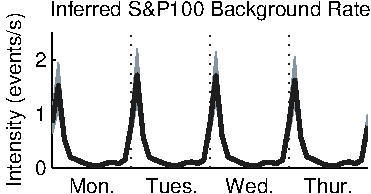
\includegraphics[width=.6\linewidth]{figures/ch2/financial_bkgd}
    \end{center}
  \end{subfigure}
  \caption[Time-varying S\&P 100 background rates]{Posterior
    distribution over shared background rates for the S\&P100. Shading
    indicates two standard deviations from the mean.}
  \label{fig:financial_bkgd}
\end{figure}

Though it is not discussed in the main text, we also considered
stochastic block model (SBM) priors as well \cite{Hoff-2008}, in hopes
of recovering latent sector affiliations based on patterns of
interaction between sectors. For example, stocks in the financial
sector may have 90\% probability of interacting with one another, and
30\% probability of interacting with stocks in the energy
sector. Rather than trying to interpret this from the embedding of a
latent distance model, we can capture this belief explicitly with a
stochastic block model prior on connectivity. We suppose there are~$J$
sectors, and the probability of belonging to a given sector
is~${\balpha \in [0,1]^J\sim\text{Dirichlet}(\balpha_0)}$. The latent
sector assignments are represented by the vector~${\bb\in [1,J]^K}$,
where~${b_k\sim\text{Cat}(\balpha)}$. The probability of a directed
interaction is~${\Pr(A_{k,k'}=1)=B_{b_{k},b_{k'}}}$, where~$\bB$ is
a~${J\times J}$ matrix of Bernoulli probabilities. We place a beta
prior on the entries of $\bB$.

Our experiments with the SBM prior yield comparable predictive
performance to the latent distance prior, as shown in
Figure~\ref{tab:financial_pred_ll_sbm}. The inferred clusters (not
shown) are correlated with the clusters identified by Bloomberg.com,
but more analysis is needed. It would also be interesting to study the
difference in inferred interactions under the various graph models;
this is left for future work.

\begin{table}
  \begin{tabular}{|l|c|}
    \hline
    \textbf{Financial Model} & \textbf{Pred. log lkhd. (bits/spike)} \\
    \hline
    Indep. LGCP & $0.579\pm 0.006$ \\
    Std. Hawkes & $0.903\pm 0.003$ \\
    Net. Hawkes (Erd\H{o}s-Renyi) & $0.893\pm 0.003$ \\
    Net. Hawkes (Latent Distance) & $0.879\pm 0.004$ \\
    Net. Hawkes (SBM) & $0.882\pm 0.004$ \\
    \hline
  \end{tabular}
  \caption[Financial model predictive log likelhioods]{Comparison of
    financial models on a event prediction task, relative to a
    homogeneous Poisson process baseline.}
  \label{tab:financial_pred_ll_sbm}
\end{table}


\section{Gangs of Chicago model details}

% Chicago cross validation
\begin{figure}[!t]
  \begin{subfigure}[T]{.24\linewidth}
    \begin{center}
      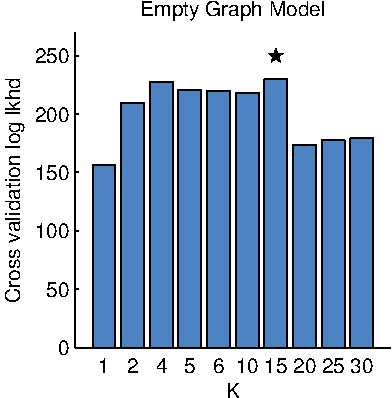
\includegraphics[width=\linewidth]{figures/ch2/icpsr_xv_empty}
    \end{center}
  \end{subfigure}
  \begin{subfigure}[T]{.24\linewidth}
    \begin{center}
      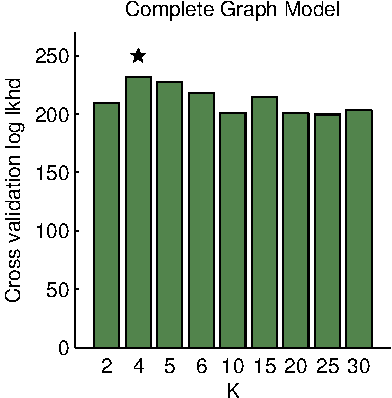
\includegraphics[width=\linewidth]{figures/ch2/icpsr_xv_complete}
    \end{center}
  \end{subfigure}
  \begin{subfigure}[T]{.24\linewidth}
    \begin{center}
      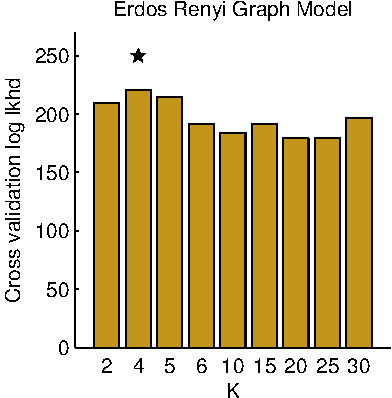
\includegraphics[width=\linewidth]{figures/ch2/icpsr_xv_er}
    \end{center}
  \end{subfigure}
  \begin{subfigure}[T]{.24\linewidth}
    \begin{center}
      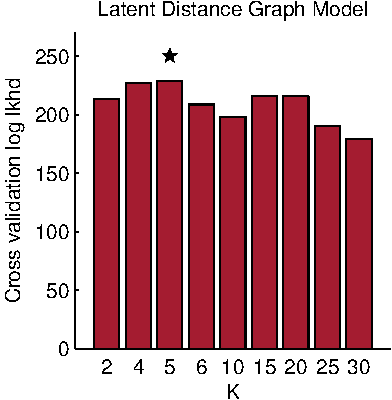
\includegraphics[width=\linewidth]{figures/ch2/icpsr_xv_dist}
    \end{center}
  \end{subfigure}
  \caption[Cross validation results for Gangs of Chicago models]{Cross
    validation results for Chicago models with~$K$ clusters for each
    of the four graph models.}
  \label{fig:chicago_xv}
\end{figure}

The first 12 years are used for training, 1993 is reserved for
cross-validation, and the remaining two years are used to test the
predictive power of the models. We also considered the crime dataset
from \url{www.data.cityofchicago.org}, but this does not identify
gang-related incidents.

We run our Markov chain for 700 iterations and use the last 200
iterations to compute predictive likelihoods and expectations. The
posterior sample illustrated in the figure in main text is the last
sample of the chain.

Since this is a spatiotemporal dataset, our intensities are functions
of both spatial location and time. For simplicity we factorize the
intensity into~${\lambda_{k,x}(\bx)\lambda_{k,t}(t)}$,
where~${\lambda_{k,t}(t)}$ is a Gaussian process as described above,
and~${\lambda_{k,x}(\bx)}$ is uniformly distributed over the spatial
region associated with process~$k$ and is normalized such that it
integrates to~$1$.

In the case of the latent distance model with the community process
model, each community's location is fixed to its center of mass. With
the cluster process model, we introduce a latent location for each
cluster and use a Gaussian distribution for the prior probability that
a community belongs to a cluster. This encourages spatially localized
clusters.

Figure~\ref{fig:chicago_xv} shows the cross validation results used to
select the number of clusters,~$K$, in the clustered process identity
model and each of the four graph models. For the empty, complete, and
Erd\"os-Renyi graph priors, we discover~${K=15}$, 4, and 4 clusters
respectively. The latent distance model, with its prior for spatially
localized clusters, has its best performance for~${K=5}$ clusters.

The spatial GMM process ID model from \citet{Cho-2013} fails on this
dataset because it assigns its spatial intensity over all
of~$\reals^2$, whereas the clustering model concentrates the rate on
only the communities in which the data
resides. Figure~\ref{fig:chicago_pred_ll_gaussian} shows the results
of this spatial process ID model on the prediction task. We did not
test a latent distance model with the spatial GMM, but it would likely
suffer in the same way as the empty, complete, and Erd\H{o}s-Renyi
graph priors.
 
\begin{figure}[!h]
  \begin{center}
    \begin{subfigure}[T]{.85\linewidth}
      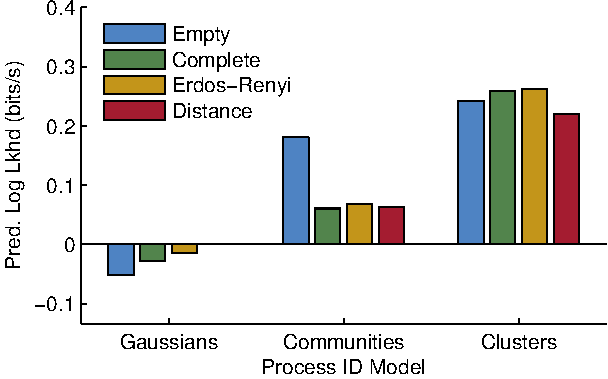
\includegraphics[width=\linewidth]{figures/ch2/icpsr_pred_ll_gaussians}
    \end{subfigure}
  \end{center}
  \caption[Extended predictive log likelihood comparison for Gangs of
    Chicago]{Comparison of predictive log likelihoods for Chicago
    homicides. This is the same as Figure~\ref{fig:chicago_predll} of
    the main text, but also includes the spatial GMM process identity
    model.}
  \label{fig:chicago_pred_ll_gaussian}
\end{figure}


